\section{\ltwotau 分析}\label{sec:1l2tau}
\ltwotau 聚焦于通过$ttH\rightarrow \tau^+\tau^-$衰变道寻找$t\bar{t}H$,其分析基本遵循文献~\cite{Aaboud:2017jvq}的方法,但是对于2015-2017年的数据分析,考虑到ATLAS对$\tau$ 的鉴别效率的提升,$\tau$ 的选择条件有一定的加强。
\ltwotau 的基本策略是经过初步的事例筛选之后(pre-MVA),利用BDTG\cite{Hocker:2007ht}方法进一步区分信号与主要本底,即$t\bar{t}$(其中至少一个$\tauhad$是来源于$b$ 喷注,强子化衰变的$W$玻色子或者部分子簇射)。
最后$0<\text{BDT}\le 0.6$和$0.6<\text{BDT}\le 1.0$为信号比例较高的区域,$\text{BDT}<0.$为信号比例较低的区域,同时拟合三个区域得到信号强度。

\subsection{事例筛选}
%轻子,喷注以及$\tauhad$的筛选跟其他衰变道一致,轻子须通过\texttt{isolationFixedCutLoose},电荷误判压低变量和non-prompt轻子压低变量。所用的单轻子触发判选条件如下:
\ltwotau 使用单轻子触发器,列出如下:
\begin{itemize}
\item 2015年数据: HLT\_mu20\_iloose\_L1MU15 || HLT\_mu50 || HLT\_e60\_lhmedium || 
 HLT\_e24\_lhmedium\_L1EM20VH || HLT\_e120\_lhloose;
\item 2016年和2017年数据: HLT\_mu26\_ivarmedium || HLT\_mu50 || HLT\_e140\_lhloose\_nod0 || 
HLT\_e26\_lhtight\_nod0\_ivarloose || HLT\_e60\_lhmedium\_nod0.\\
%\item The trigger lepton is required to have: pT$>27$ GeV/c in 2016 and 2017 data; pT$>21$ GeV/c for muon and 25 GeV/c for electron in 2015 data.
\end{itemize}
在2016年和2017年数据中要求触发轻子\pT$>27$ GeV,2015年数据中要求触发电子\pt$>25$ GeV,,$\mu$子\pt$>21$ GeV。
%喷注\pt 要求至少25 GeV,$|\eta|<2.5$,以及\texttt{JVT}条件。\btag 是基于多变量学习方法的,所选的\btag 效率WP为70\%,\ltwotau 要求所有喷注都不是\btagged 的。
%$\tauhad$须通过\texttt{tight} ID,\pt$>$25 GeV以及$|\eta|<2.5$筛选,其中$1.37<|\eta|<1.52$,即电磁量能器的空区,被排除掉。\\

根据章节\ref{sec:obj_tth}所述筛选粒子,轻子还须通过\texttt{isolationFixedCutLoose}。
%注意到\ltwotau 中的主要本底是$t\bar{t}$,可以通过加强粒子筛选条件压低此项本底:
%\begin{enumerate}
% \item 因为至少一个$\tauhad$是来自$b$ 喷注,所以要求所选的$\tauhad$不是\btagged 的,可以去除25\%的假本底,而保持96\%的信号选择效率;
%  \item 喷注数和$\tauhad$ \pt 可以帮助压低假本底,这是因为$t\bar{t}$倾向具有较少的喷注数和较低动量的$\tauhad$;
%   但是它们作为BDTG的训练变量也许能够发挥更大作用,所以选择具有至少三个喷注和$\tauhad$ \pt 大于25 GeV的事例。%,与其他衰变道一致。
%\end{enumerate}
而后根据如下条件进行初步事例筛选:
\begin{itemize}
  \item 两个通过\texttt{tight} ID具有相反电荷的$\tauhad$,\pt$>$25 GeV,并且都没有\btagged;
  \item 两个$\tauhad$必须来自初始顶点;
  \item 一个匹配任一触发判选条件的孤立电子或$\mu$子;
  \item 至少三个喷注,其中至少一个是\btagged 的。
\end{itemize}

\subsection{Fakes本底估计}
虽然利用多变量学习方法构建的$\tauhad$ ID能够过滤掉大部分假$\tauhad$,但是在\ltwotau 的主要本底仍然是假$\tauhad$。
另外,通过检查所选轻子的来源,发现接近99\%是真实的。所以,只需估计假$\tauhad$即可。通过检查MC可以对假$\tauhad$来源有一定的了解,
定义来自希格斯玻色子或者矢量玻色子的为真(real)$\tauhad$,来自QCD喷注的为假(fake)$\tauhad$。
图\ref{Fig:1l2tau.truth}中两$\tauhad$分为fake-fake,fake-real,来自于$H\rightarrow \tau\tau$
的real-real,以及其他;可以发现$t \bar{t}h$ 的纯度非常高,达到90\%,而主要来源于$t\bar{t}$的本底至少有一个fake。
图\ref{Fig:1l2tau.truth}也给出假$\tauhad$的来源分布,大部分来源胶子喷注。由图中还可以发现相反电荷与相同电荷具有非常相似的分布,
这给随后的假$\tauhad$估计方法给予一定的支持。
%其稍微的不同会考虑成假本底的形状误差,通过比较相同电荷与相反电荷的$t\bar{t}$样本得到,这会在章节\ref{sec:1l2tau_sys}中讨论。
\begin{figure}[htbp]
\centering
\begin{center}
  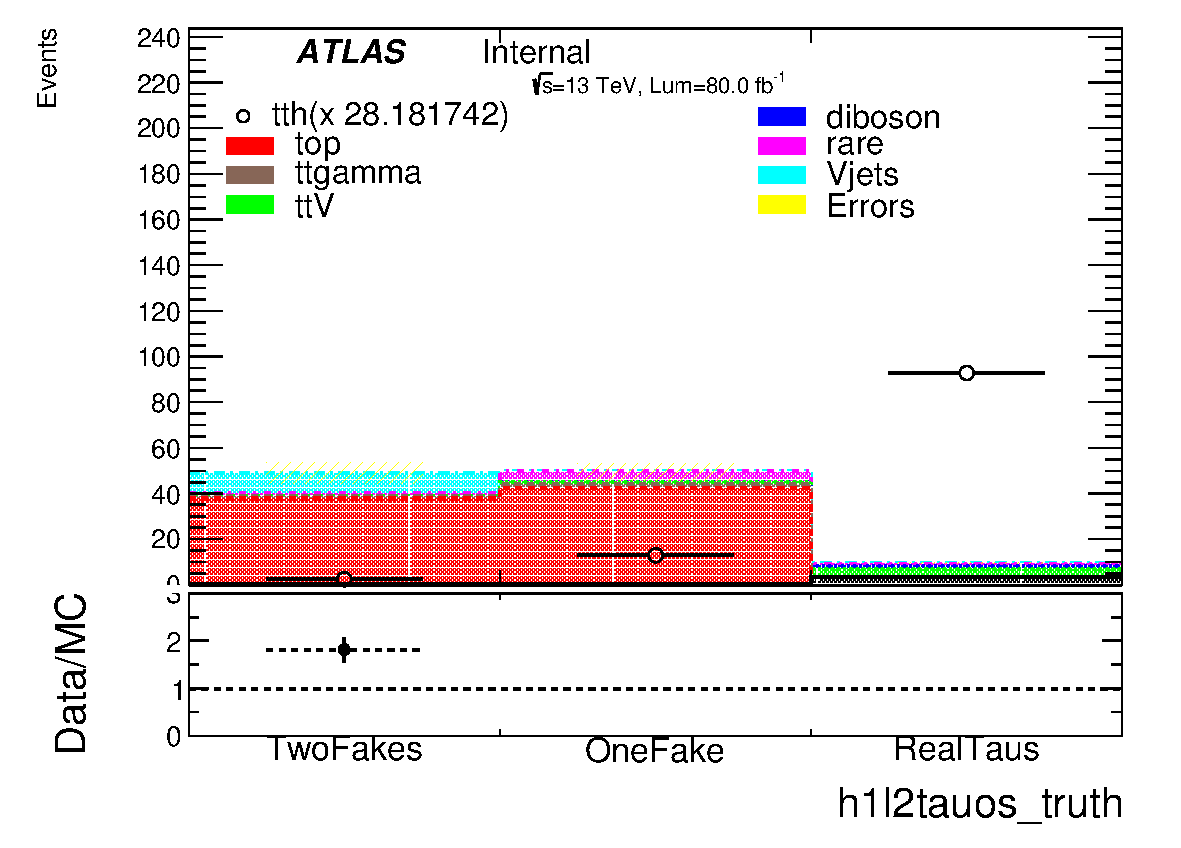
\includegraphics[width=0.45\textwidth, keepaspectratio]{fig/OneLepTwoTaus/Plots_h1l2tauos_truth_signal.pdf}
  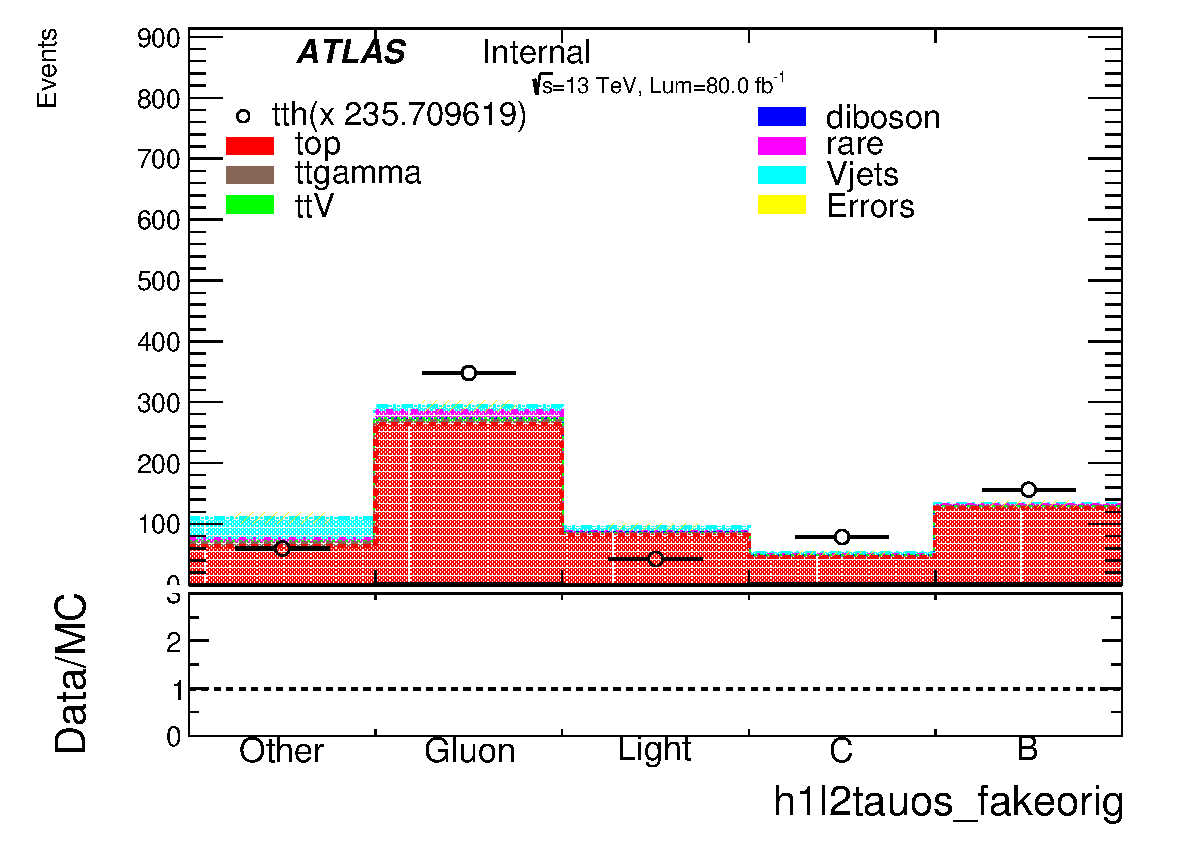
\includegraphics[width=0.45\textwidth, keepaspectratio]{fig/OneLepTwoTaus/Plots_h1l2tauos_fakeorig_signal.pdf}
  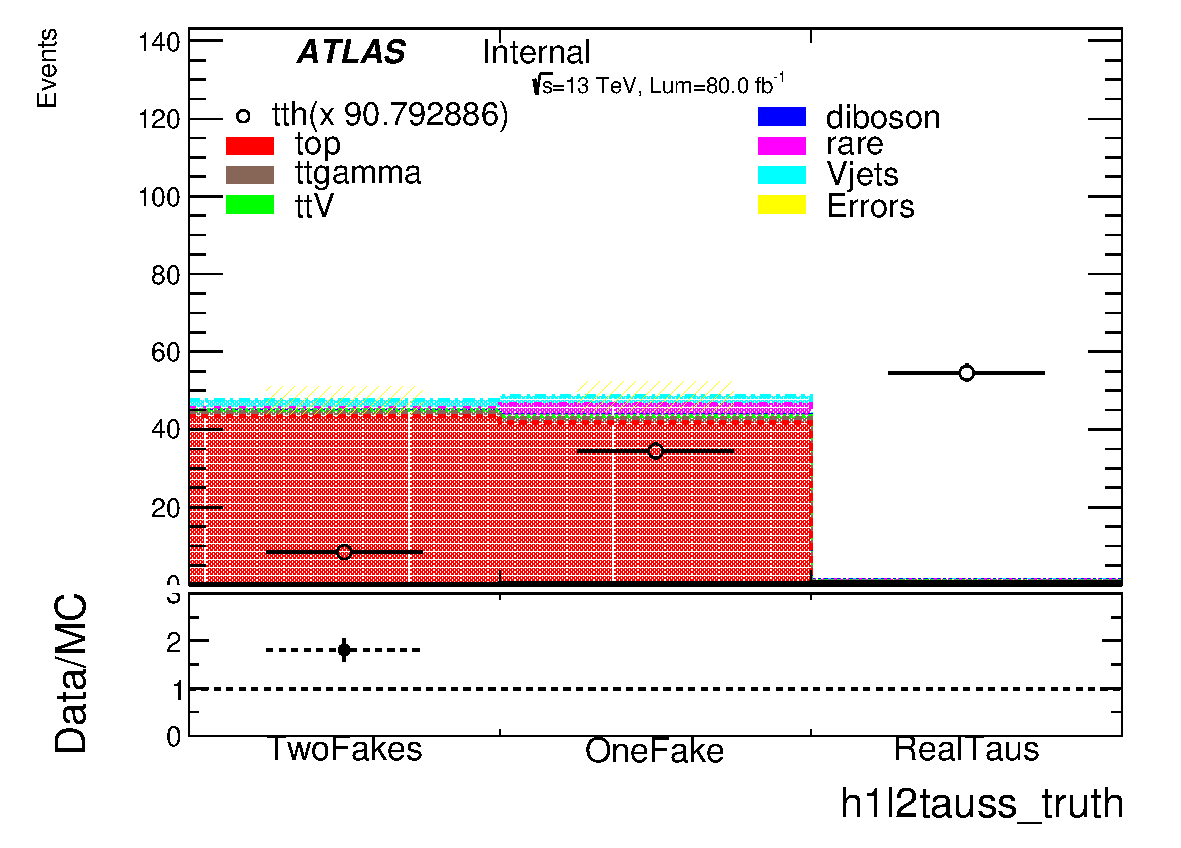
\includegraphics[width=0.45\textwidth, keepaspectratio]{fig/OneLepTwoTaus/Plots_h1l2tauss_truth_signal.pdf}
  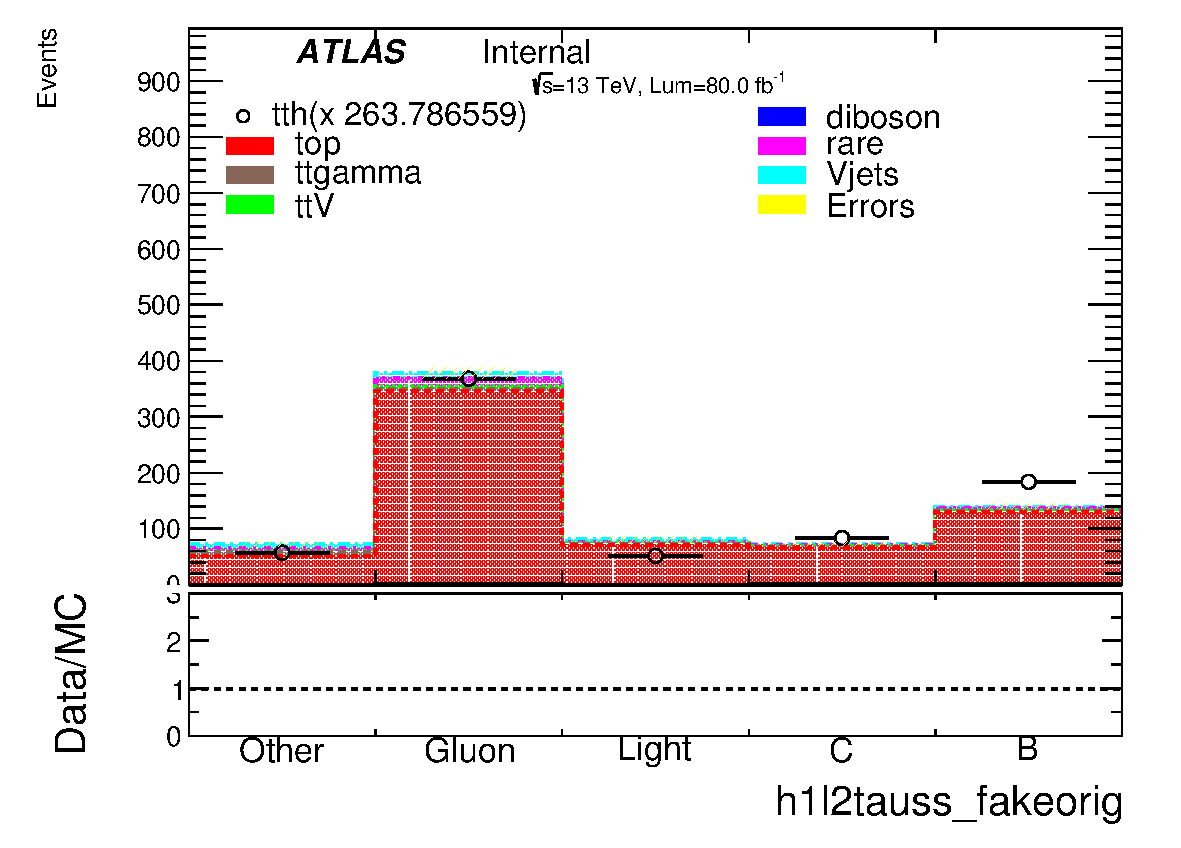
\includegraphics[width=0.45\textwidth, keepaspectratio]{fig/OneLepTwoTaus/Plots_h1l2tauss_fakeorig_signal.pdf}
\end{center}
\caption{左列展示根据MC真实信息双$\tau_{\text{had}}$事例分为fake-fake, fake-real, real-real和其他的分布,右列展示假$\tau_{\text{had}}$的来源分布,第一行对应SS双$\tau_{\text{had}}$,第二行对应OS双$\tau_{\text{had}}$。}
%\caption{The original di-tau events are classified based on the Monte Carlo truth as fake-fake, fake-real, real-real from Higgs decay or 
%anything else, respectively, in left and the origin of the fake taus are shown in right. The top row for OS and the bottom row for SS. The signal is normalized to the total background in each plot.}
\label{Fig:1l2tau.truth}
\end{figure}

虽然MC在一定程度上可以帮助对假$\tau_{\text{had}}$的理解,但是它并不能很好描述假$\tau_{\text{had}}$,利用data-driven方法\footnote{data-driven表示利用数据去估计本底的一类方法。}去估计$\tau_{\text{had}}$是非常有必要的。\\
喷注被误判成$\tau_{\text{had}}$时,其有相同概率被标定成带正电或者负电,所以,假本底中相同电荷(SS)两$\tau_{\text{had}}$和相反电荷(OS)两$\tau_{\text{had}}$事例比例应该相当。
这样,可以利用SS数据去估计OS信号区的假本底,即:
\begin{equation}
 \begin{aligned}
  \text{Expected fakes}: \text{OS}_{\text{fake}}=\text{SS}_{\text{data}}-\text{SS}_{\text{truth}}\\
  \text{Expected total yield}: \text{OS}_{\text{exp}}=\text{OS}_{\text{fake}}+\text{OS}_{\text{truth}}
 \end{aligned}
\end{equation}
其中,$\text{OS}/\text{SS}_{\text{data}}$是观测到的数据中的OS/SS事例数,$\text{OS}/\text{SS}_{\text{truth}}$则是MC中(包括信号MC)真实$\tau_{\text{had}}$事例数。
表\ref{Tab:1l2tau.fake}在两个控制区验证此假设,分别是低信号区($\text{BDT}<0.5$, $\text{njet}>3$)和低喷注区($\text{njet}<3$),总体而言,总期望值与OS数据是一致的,最大的偏差在低信号区,
$\text{OS}_{\text{exp}}/\text{OS}_{\text{data}}$为$1.00\pm 0.22$,22\%将作为此假本底估计方法的内禀误差(closure test)。

\begin{table}[htbp]
\small
\begin{center}\scalebox{0.8}{
\begin{tabular}{c|c|c|c|c|c|c}\hline
Samples & $\text{SS}_{\text{data}}$  & $\text{SS}_{\text{truth}}$ & $\text{OS}_{\text{truth}}$ & $\text{OS}_{\text{exp}}$ & $\text{OS}_{\text{data}}$ & $\text{OS}_{\text{exp}}/\text{OS}_{\text{data}}$ \\ \hline
$\text{njet}<3$ & 112$\pm$11 & 1.2$\pm$0.1 & 10.8$\pm$1.0 & 121.6$\pm$11.0 & 108 &  1.13$\pm$0.10 \\
$\text{njet}\ge3, \text{BDT}<0.5$ & 62$\pm$7.8 & 0.55$\pm$0.07 & 4.69$\pm$0.18 & 66.1$\pm$7.9 & 54 & 1.22$\pm$0.15 \\ \hline 
%$njet\ge3,(BDT<0.5)$ & 97$\pm$9.8 & 1.33$\pm$0.08 & 9.36$\pm$0.37 &105.0$\pm$10.0 & 111$\pm$10.5 & 0.95$\pm$0.13 \\ \hline
\end{tabular}}
\caption{假$\tau_{\text{had}}$估计方法在低喷注数区和低信号区的closure test。}
%\caption{ A closure of the  data driven fake estimation is tested in the $njet<3$ and the signal depleted control regions.}
\label{Tab:1l2tau.fake}
\end{center}
\end{table}

\subsection{MVA研究}
多变量方法(MVA)可以进一步压低$t\bar{t}$本底,作为训练变量的7个运动学变量如下:
\begin{itemize}
 \item Njets: 喷注数(若大于5则设为5);
 \item Nbjets: 标定为$b$的喷注数(若大于3则设为3);
 \item Htjets: 喷注\pt 的标量和(MeV);
 \item LeadPt: 高动量$\tauhad$ \pt (GeV);
 \item SubPt: 低动量$\tauhad$ \pt (GeV);
 \item Mtautau: 两$\tauhad$不变质量(GeV);
 \item Jjdr: 所选喷注的两两组合中的最小$\Delta R$;
 \item Etamax: 两$\tauhad$中的较大$|\eta|$。
\end{itemize}
这些变量的分布如图~\ref{Fig:1l2tau.bdtinputs}所示,可以看到每个变量的区分度一般,并不足以支持应用一个简单的筛选条件,所以把这些变量输入BDTG,希望能够充分
开发其筛选潜能,提高信号显著性。
在训练中,所选信号的两$\tauhad$均是真实的,而为了增加本底事例数,$t\bar{t}$ MC包括OS和SS,总共有8258个信号事例与1268个本底事例。值得指出的是,根据事例标签,
信号MC分为奇事例与偶事例,通过奇(偶)事例得到的训练配置在实际使用中会应用到偶(奇)事例中,这样可以避免训练偏差。从图~\ref{Fig:1l2tau.bdt}看到,训练分布与测试
分布是非常接近的,说明没有过度训练。表\ref{Tab:1l2tau.bdtrank}给出输入变量的重要性排序,Etamax具有最高的重要性。在图~\ref{Fig:1l2tau.bdt}还可以看到本底压低随信号效率变化的曲线。
那么在该分析,可以直接应用一个简单的BDT筛选或者拟合BDT分布去提高信号显著性,但一般来讲,联合拟合多个信号区会给出更高的信号显著性。所以,根据BDT分为三个信号区域:$0.6<\text{BDT}\le 1.0$,
$0<\text{BDT}\le 0.6$和$\text{BDT}<0.$,最后的统计分析会联合拟合这三个区域得到最终的信号强度。\\
值得注意的是,以上多变量训练使用的本底是$t\bar{t}$ MC,而在实际的分析中,主要本底是SS data,图~\ref{Fig:1l2tau.ssbdtvalidation}比较SS data与$t\bar{t}$MC的差异,基本上,输入
变量以及BDT的分布是非常相似的。最后,表~\ref{Tab:1l2tau.summary}总结了三个信号区的事例数以及预期信号强度。
\begin{figure}[htbp]
\centering
\begin{center}
  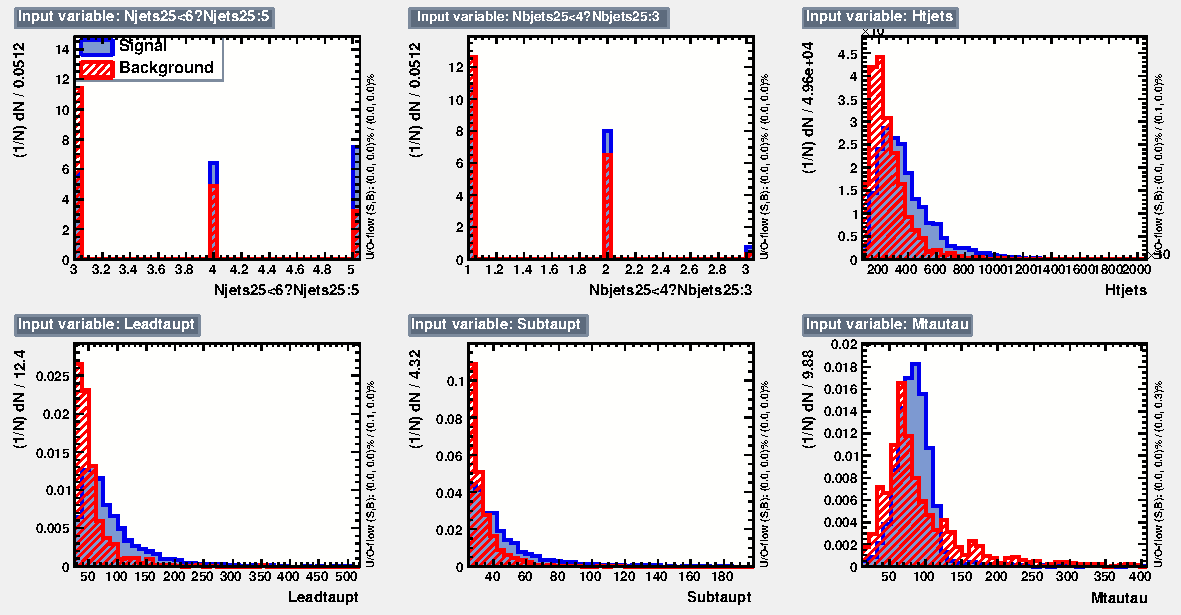
\includegraphics[width=0.8\textwidth, keepaspectratio]{fig/OneLepTwoTaus/variables_id_c1.pdf}
  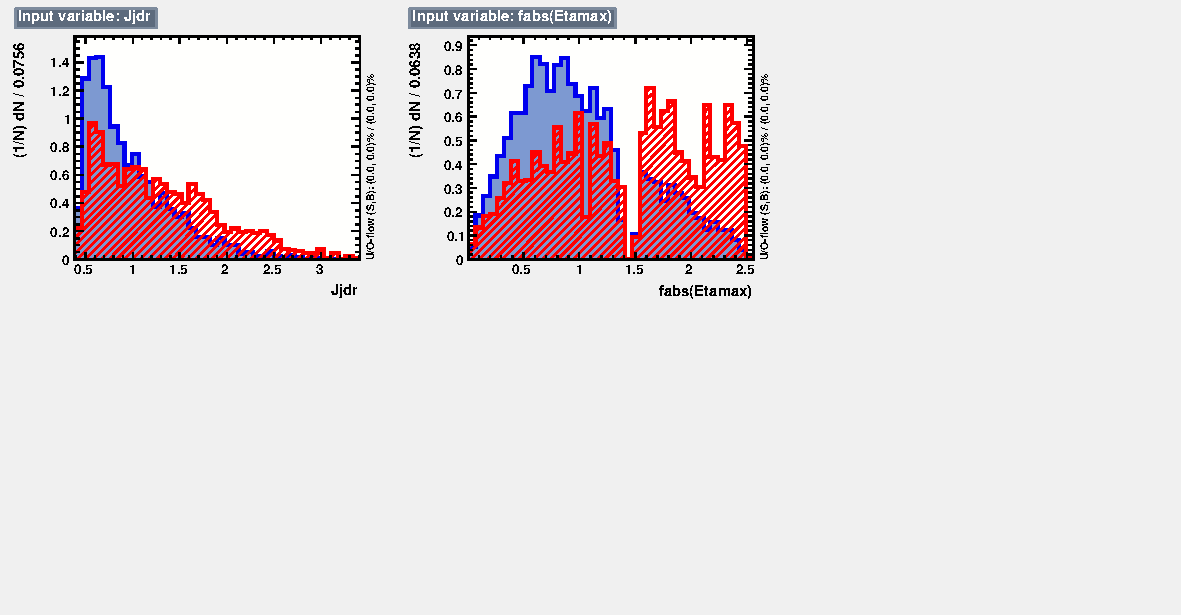
\includegraphics[width=0.8\textwidth, keepaspectratio]{fig/OneLepTwoTaus/variables_id_c2.pdf}
\end{center}
\caption{第一行: njet, nbjet, Htjets; 第二行: LeadPt, SubPt, Mtautau; 第三行: Jjdr, Etamax.}
%\caption{BDT input variables. Top row: njet, nbjet, Htjets; Middle row: LeadPt, SubPt, Mtautau;
%Bottom row: Jjdr and Etamax.}
\label{Fig:1l2tau.bdtinputs}
\end{figure}

\begin{figure}[htbp]
\centering
\begin{center}
  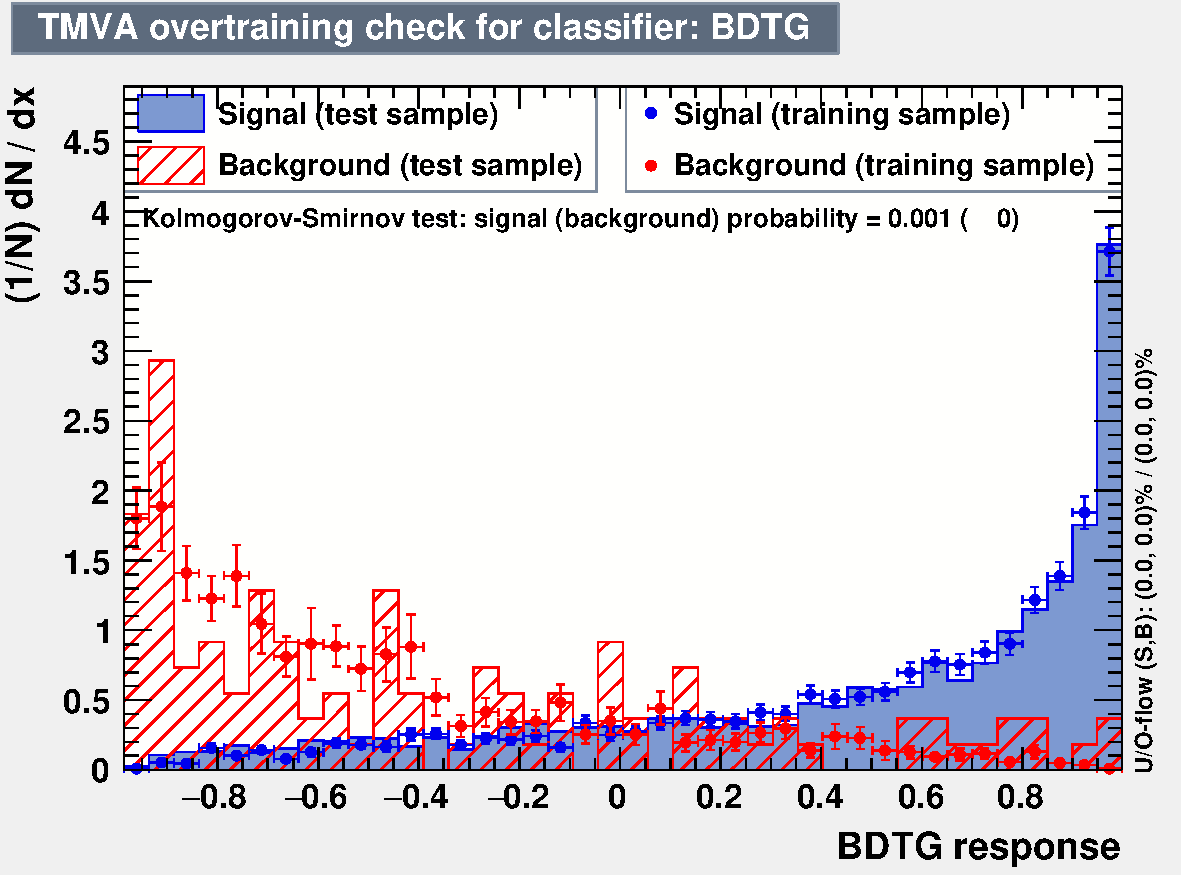
\includegraphics[width=0.45\textwidth, keepaspectratio]{fig/OneLepTwoTaus/overtrain_BDTG.pdf}
  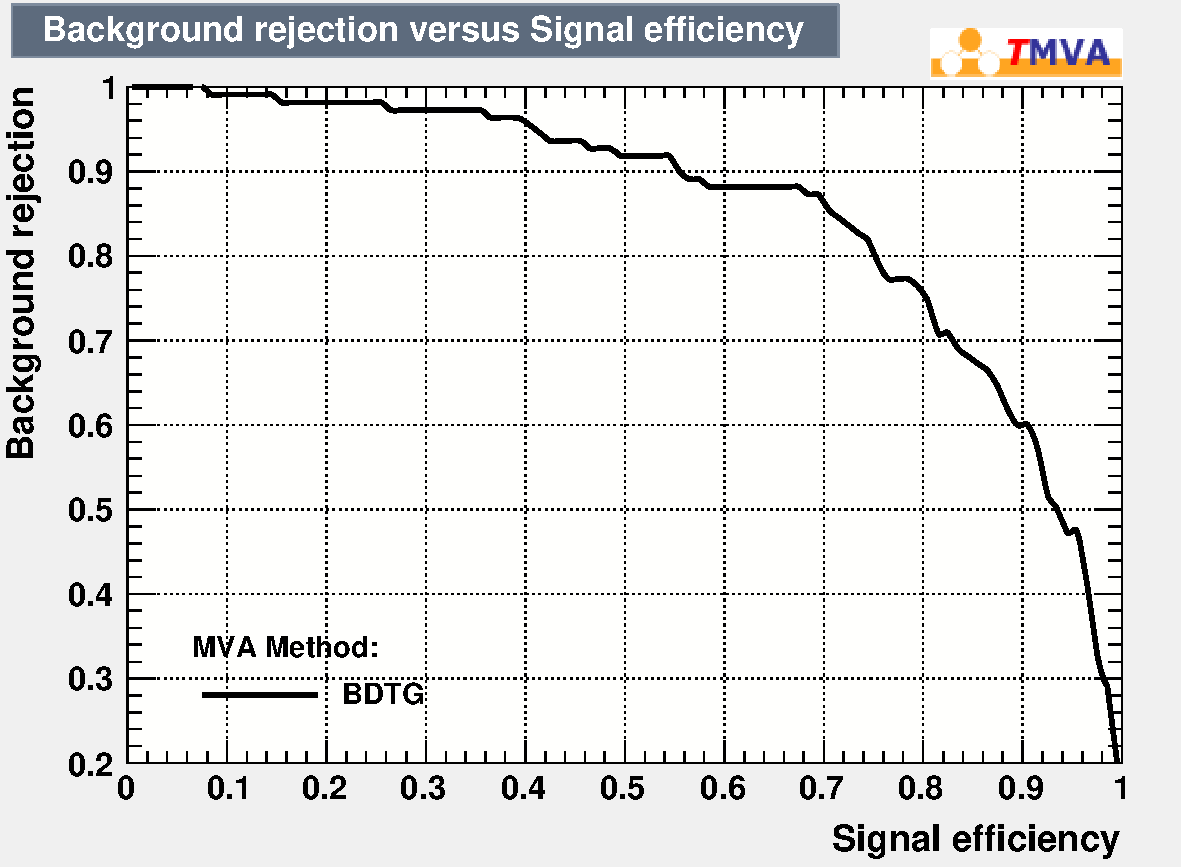
\includegraphics[width=0.45\textwidth, keepaspectratio]{fig/OneLepTwoTaus/rejBvsS.pdf}
\end{center}
\caption{左图:BDTG过度训练检查;右图:BDTG本底排除效率随信号效率分布。}
%\caption{The BDT distributions for the signal and background obtained during the training and testing (left);
%The rejection for the background vs the efficiency for the signal as a function of BDT cut (right).}
\label{Fig:1l2tau.bdt}
\end{figure}

\begin{figure}[htbp]
\centering
\begin{center}
  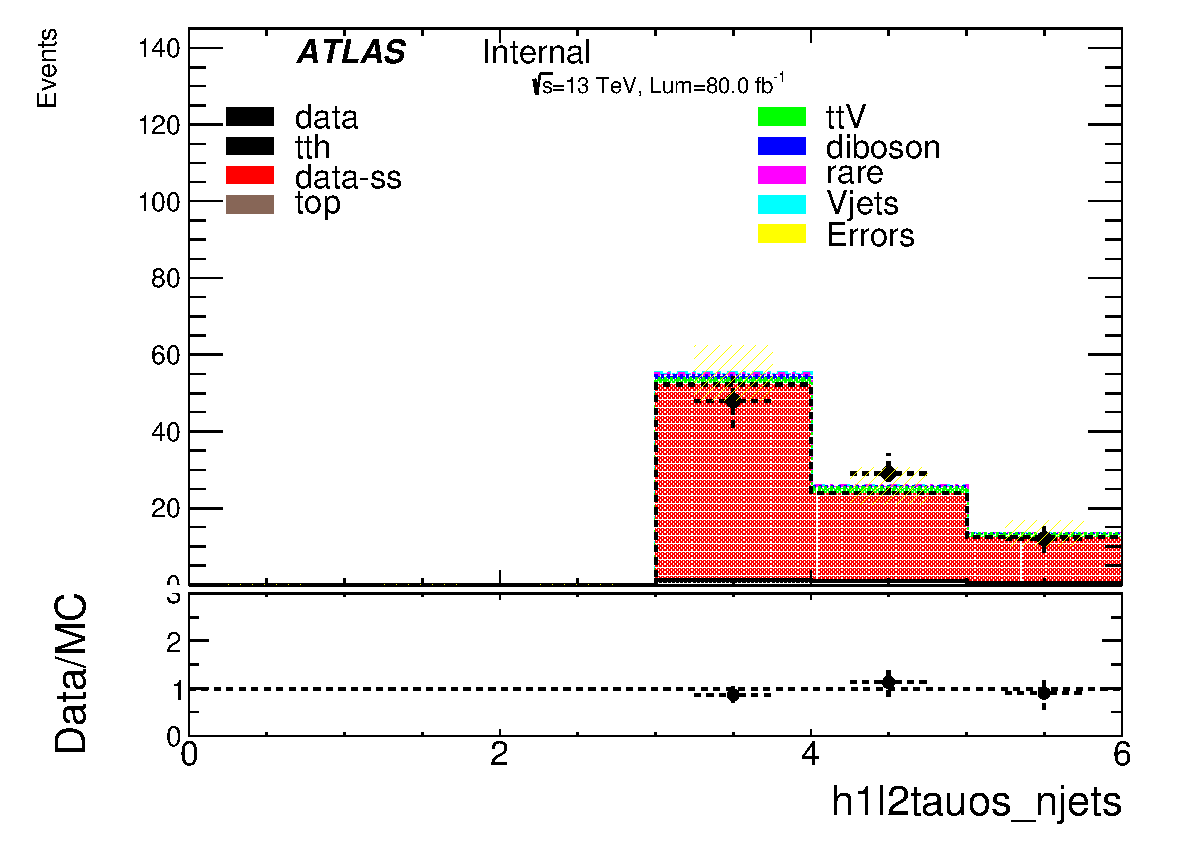
\includegraphics[width=0.3\textwidth, keepaspectratio]{fig/OneLepTwoTaus/Plots_Plots_njets_ssdata_signal.pdf}
  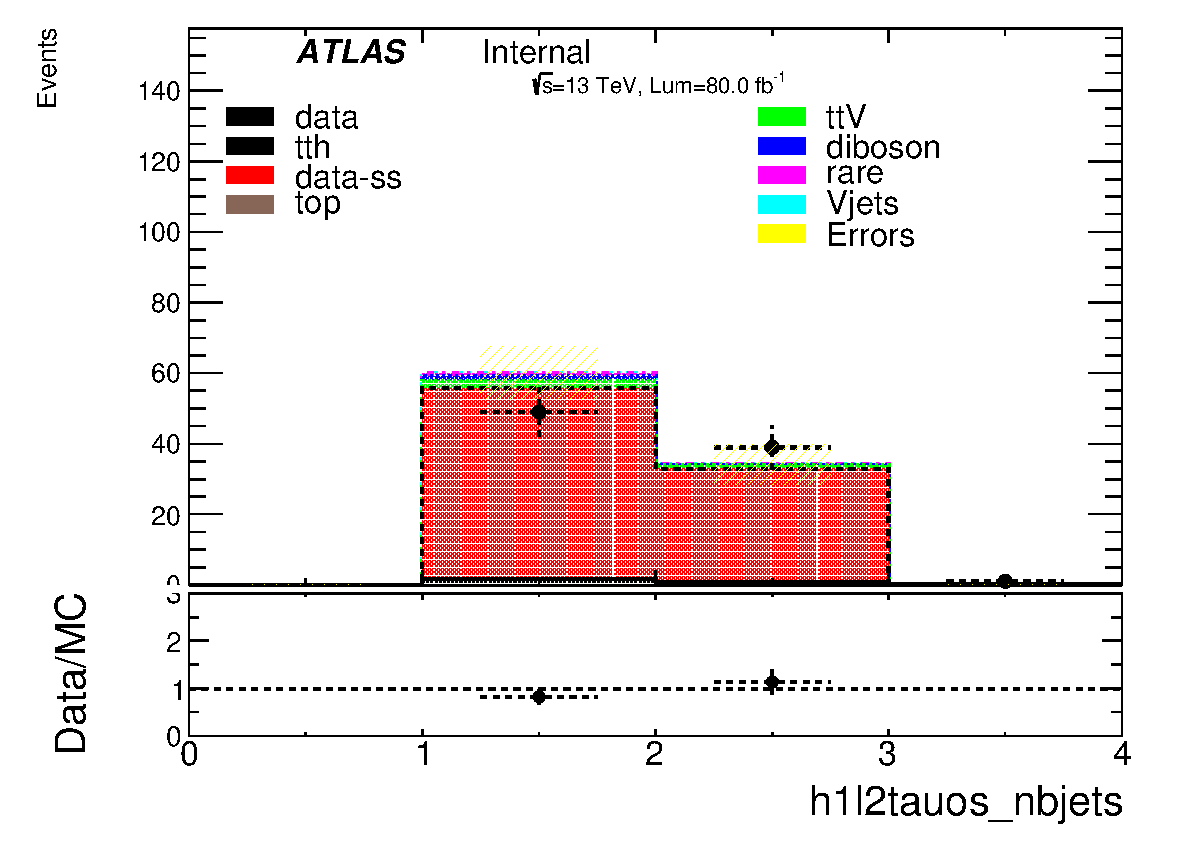
\includegraphics[width=0.3\textwidth, keepaspectratio]{fig/OneLepTwoTaus/Plots_Plots_nbjets_ssdata_signal.pdf}
  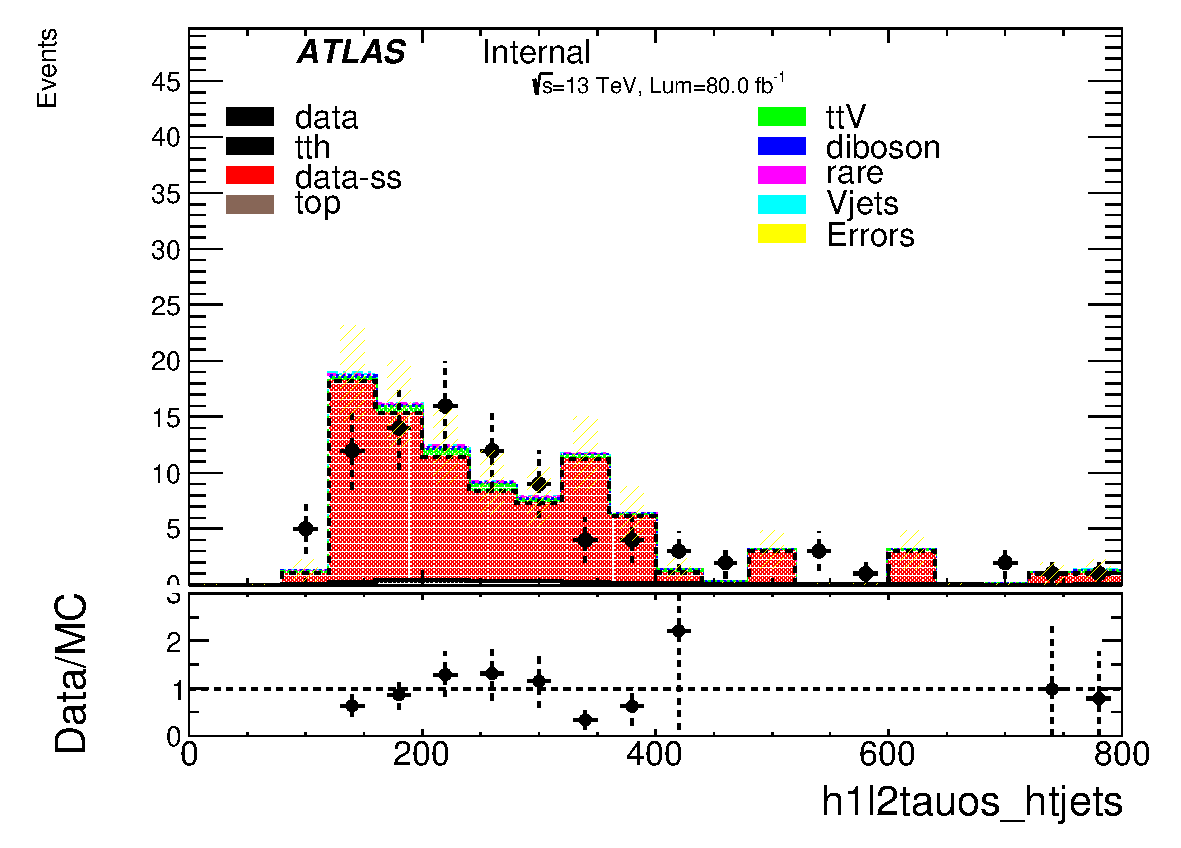
\includegraphics[width=0.3\textwidth, keepaspectratio]{fig/OneLepTwoTaus/Plots_Plots_htjets_ssdata_signal.pdf}
  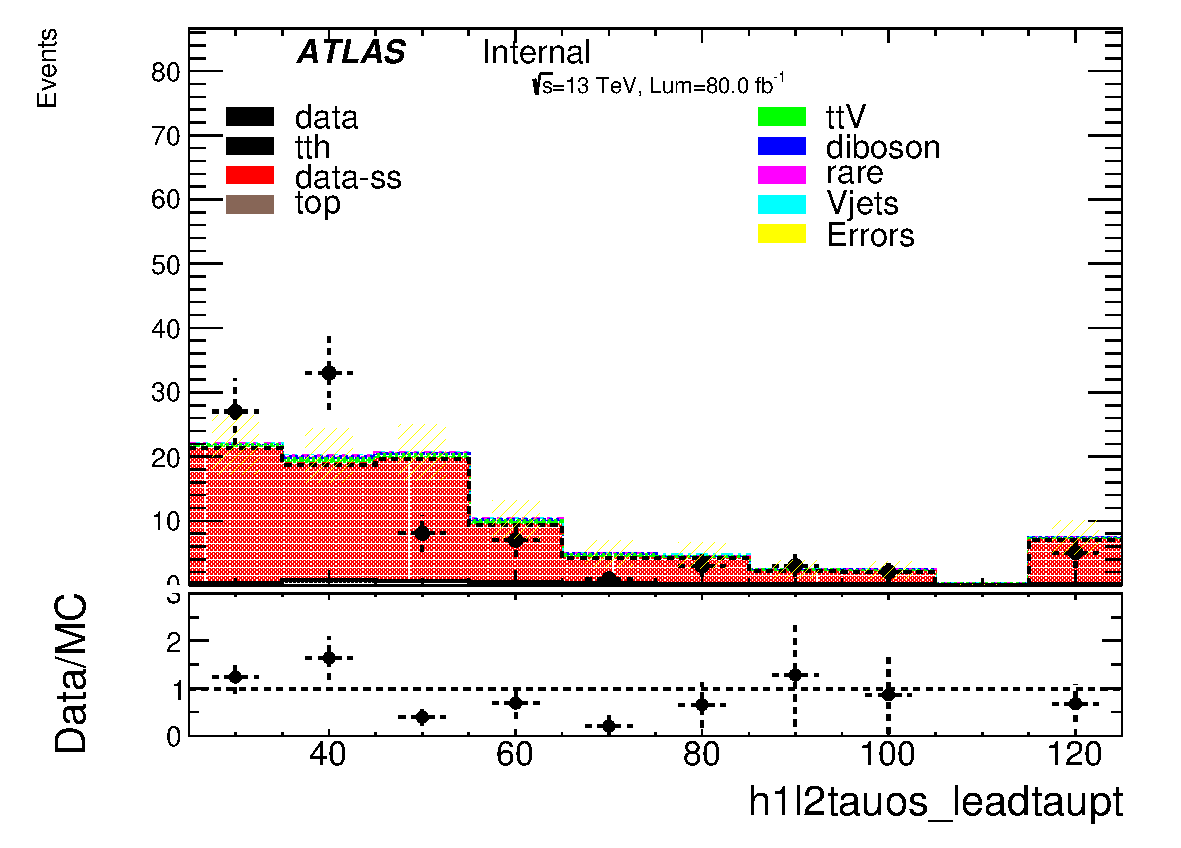
\includegraphics[width=0.3\textwidth, keepaspectratio]{fig/OneLepTwoTaus/Plots_Plots_leadtaupt_ssdata_signal.pdf}
  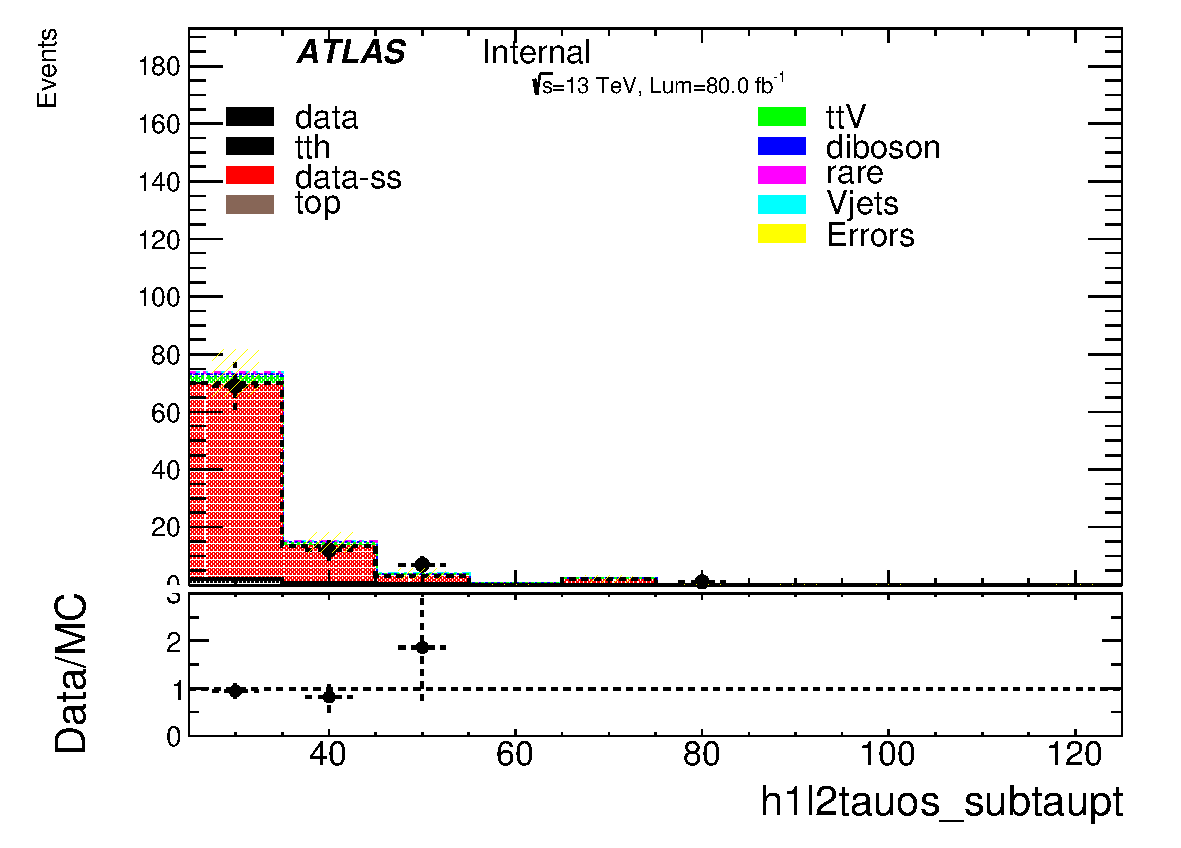
\includegraphics[width=0.3\textwidth, keepaspectratio]{fig/OneLepTwoTaus/Plots_Plots_subtaupt_ssdata_signal.pdf}
  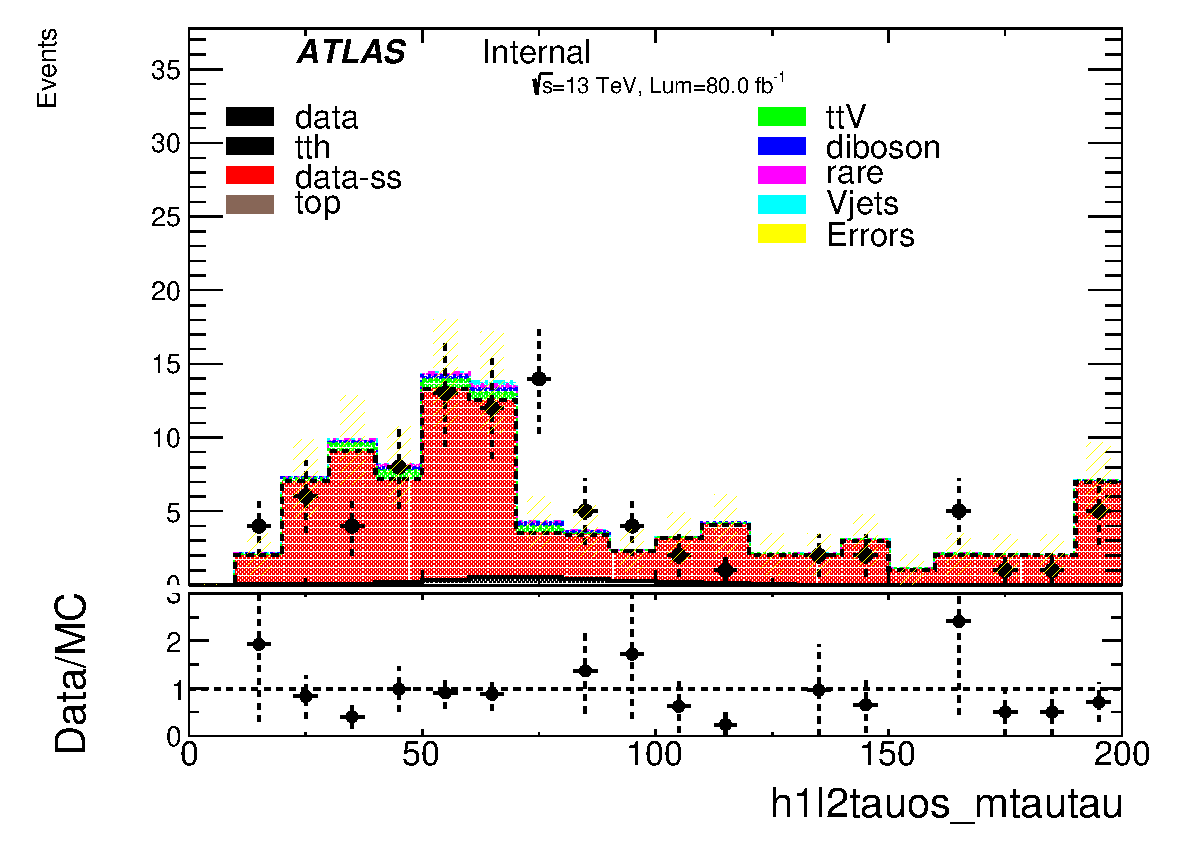
\includegraphics[width=0.3\textwidth, keepaspectratio]{fig/OneLepTwoTaus/Plots_Plots_mtautau_ssdata_signal.pdf}
  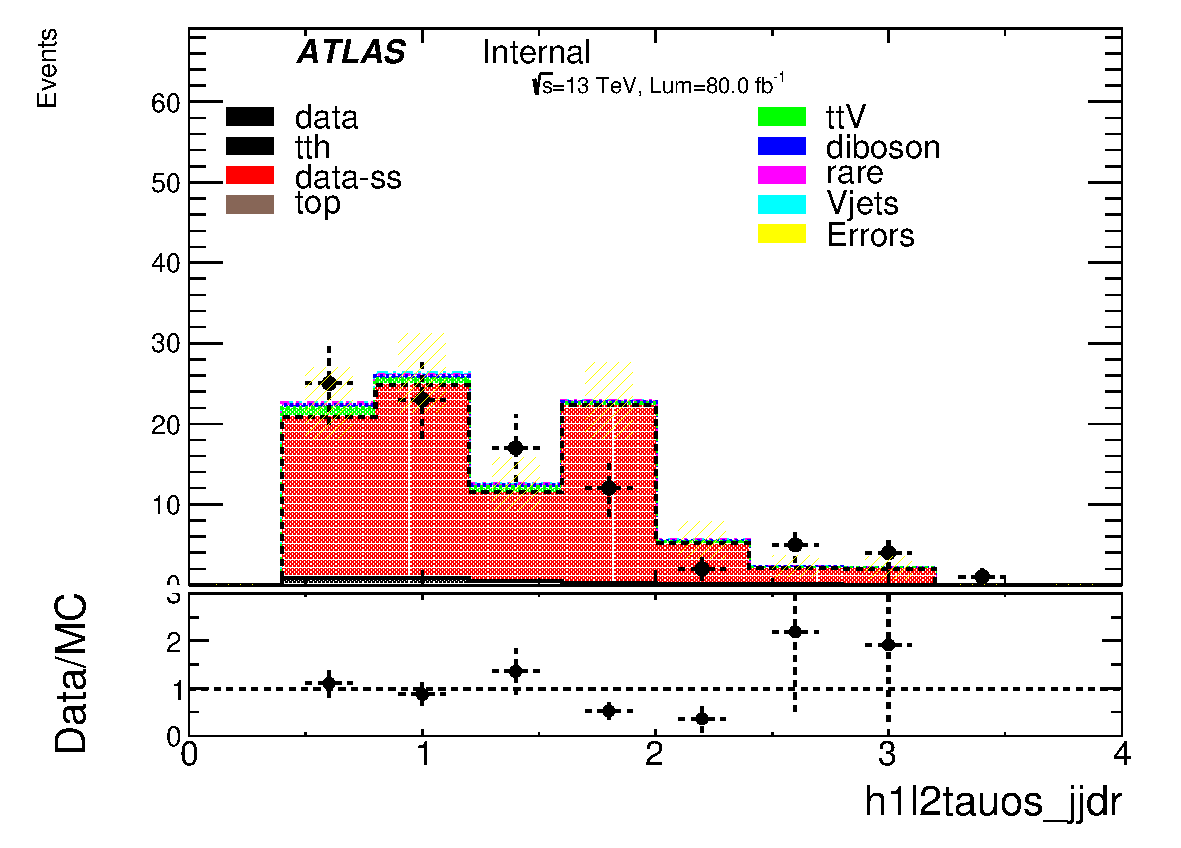
\includegraphics[width=0.3\textwidth, keepaspectratio]{fig/OneLepTwoTaus/Plots_Plots_jjdr_ssdata_signal.pdf}
  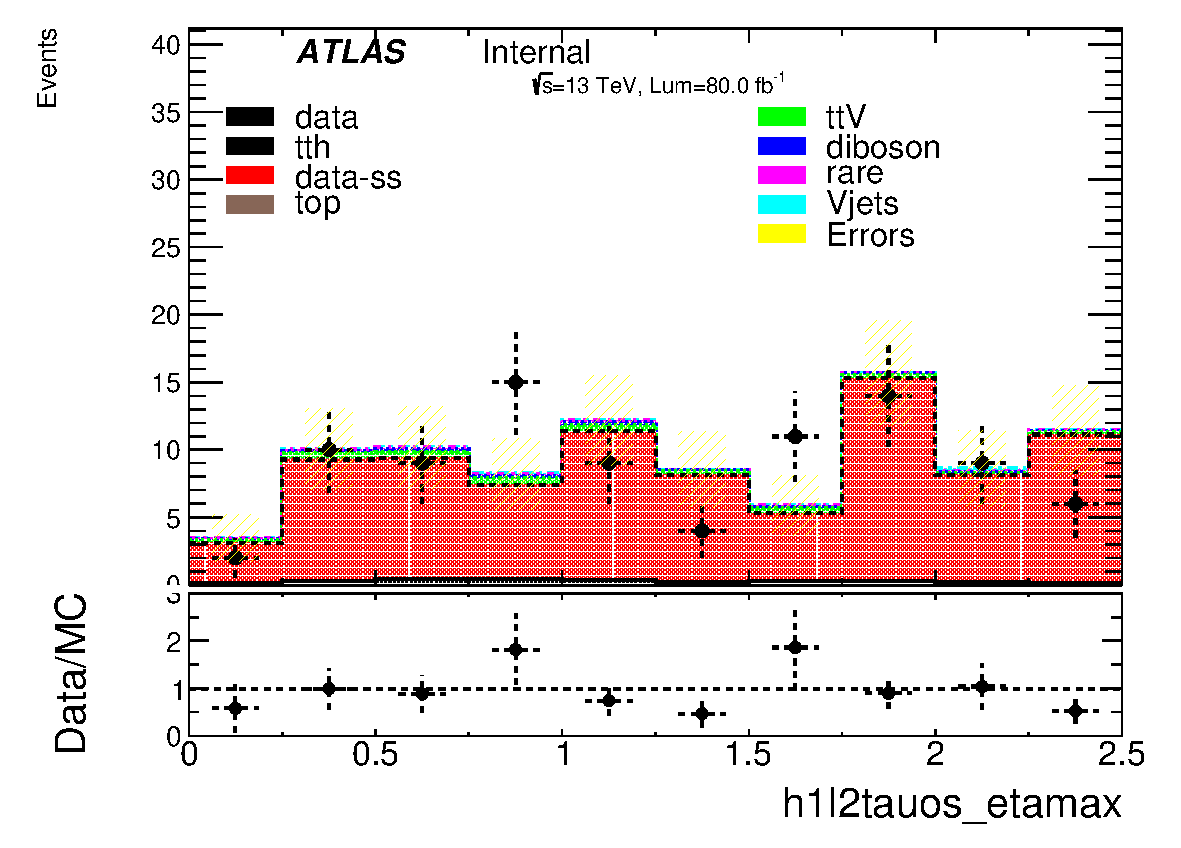
\includegraphics[width=0.3\textwidth, keepaspectratio]{fig/OneLepTwoTaus/Plots_Plots_etamax_ssdata_signal.pdf}
  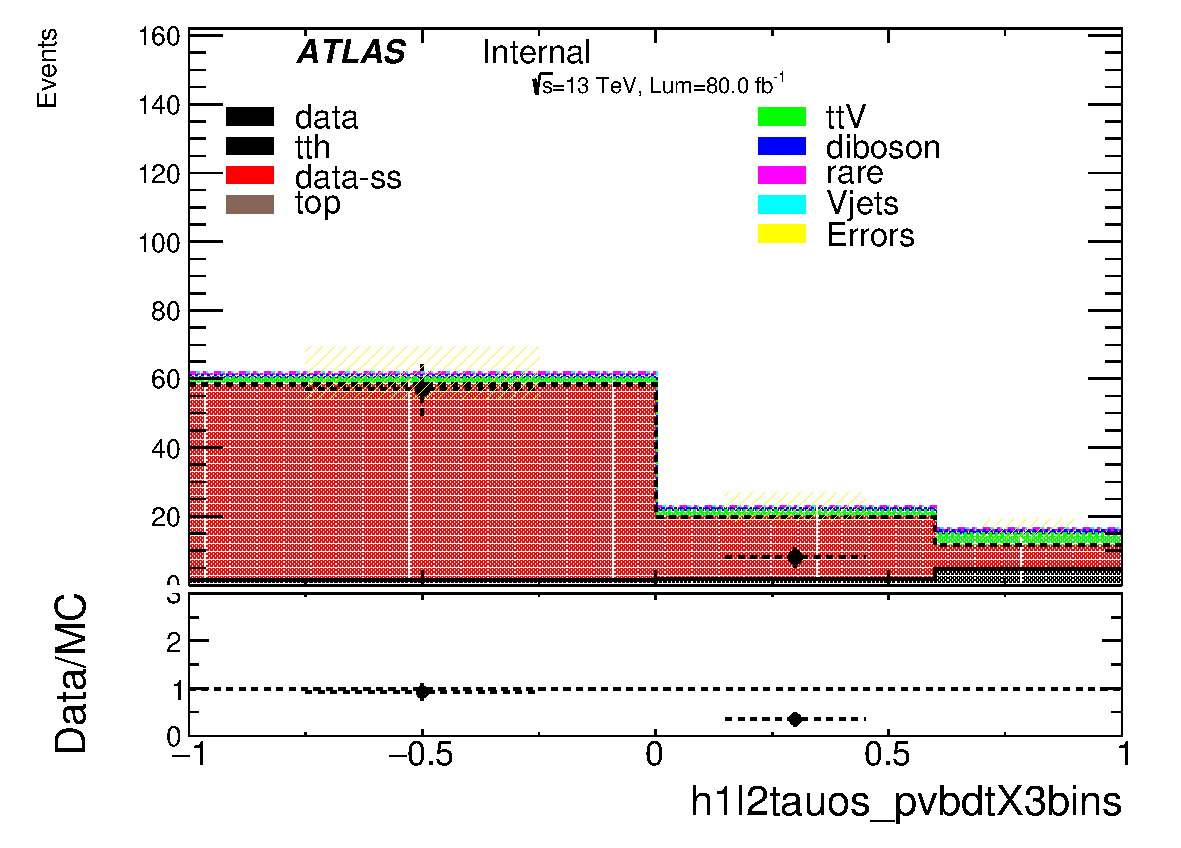
\includegraphics[width=0.3\textwidth, keepaspectratio]{fig/OneLepTwoTaus/Plots_Plots_bdtT3bins_ssdata_signal.pdf}
\end{center}
\caption{SS信号区数据与预期本底比较,第一行: njet, nbjet, Htjets; 第二行: LeadPt, SubPt, Mtautau; 第三行: Jjdr, Etamax, BDT.}
%\caption{The BDT inputs and output are compared using the SS events in the signal region.
%Top row: njet, nbjet; Second row: Htjets, leadPt; Third row: subPt, mtautau; Bottom row: Jjdr, Etamax, and BDT.
%({\bf update from tth fitter including systematics})
%}
\label{Fig:1l2tau.ssbdtvalidation}
\end{figure}

\begin{table}[htbp]
\begin{center}
\begin{tabular}{c|c|c}\hline
Rank & Input variable  & Importance \\ \hline
1 & Etamax & 0.18\\
2 & Mtautau & 0.15 \\
3 & Jjdr & 0.14 \\
4 & Htjets & 0.13 \\
5 & LeadPt & 0.125 \\
6 & SubPt & 0.12 \\
7 & Njets & 0.089 \\
8 & Nbjets & 0.068 \\ \hline
\end{tabular}
\caption{训练变量重要性排名。}
%\caption{ The rank of input variables are shown based on their improtance to BDT.}
\label{Tab:1l2tau.bdtrank}
\end{center}
\end{table}

\begin{table}[htbp]
\begin{center}
\begin{tabular}{c|c|c|c|c}\hline
OS Sample & $\text{BDT}\le0.$  & $0<\text{BDT}\le 0.6$ & $0.6<\text{BDT}\le 1.0$ & Total \\ \hline
ttH(truth) & 1.25$\pm$0.19 & 1.71$\pm$0.25 & 4.17$\pm$0.98 & 7.13$\pm$1.34 \\
ttV(truth) & 1.65$\pm$0.29 & 1.62$\pm$0.31 & 3.03$\pm$0.52  & 6.31$\pm$1.02\\
Diboson(truth) & 0.70$\pm$0.39 & 0.48$\pm$0.26 & 0.72$\pm$0.39 & 1.90$\pm$1.01\\
Rare(truth) & 0.09$\pm$0.05 & 0.09$\pm$0.05 & 0.19$\pm$0.10 & 0.36$\pm$0.19\\
Fake(SS) & 50.0$\pm$13.1 & 15.0$\pm$5.1 & 5.0$\pm$2.5 & 70.0$\pm$17.5\\
Total B & 52.4$\pm$13.1 & 17.2$\pm$5.1 & 8.9$\pm$2.6 & 78.6$\pm$17.6\\ \hline
$z_0$ & 0.09 & 0.23 & 0.73 & 0.98\\ \hline
%ttH(truth) & $1.29\pm 0.05$ & $2.04\pm 0.07$ & $4.82\pm 0.10$ & $8.14\pm 0.13$\\ \hline
%ttV(truth) & $1.82\pm 0.14$  & $1.89\pm 0.14$ & $3.48\pm 0.19$& $7.18\pm 0.28$ \\
%Dibison(truth) & $0.85\pm 0.09$ & $0.59\pm 0.06$ & $0.84\pm 0.07$ & $2.28\pm 0.13$ \\
%top(truth) & $0.25\pm 0.23$  & $0.03\pm 0.03$ & $0\pm 0$ & $0.28\pm 0.23$\\
%Rare(truth) & $0.07\pm 0.02$  & $0.07\pm 0.02$ & $0.18\pm 0.03$ &  $0.32\pm 0.04$\\
%Vjets(truth) & $0.20\pm 0.20$  & $0.03\pm 0.03$ & $0\pm 0$ &$0.23\pm 0.20$\\
%Fake(SS) & $82\pm 9.0$ & $16\pm 4$ & $12\pm 3$ & $110\pm 10.5$\\ \hline
%Total B & $85.20\pm 9.10$ & $18.60\pm 4.00$ & $16.50\pm 3.50$ &$120.30\pm 10.50$\\ \hline
%$z_0$ & 0.14 & 0.46 & 1.13 &0.73 \\ \hline
\end{tabular}
\caption{预期信号与本底数。}
%\caption{ The summary of signal and backgrounds in the three categories entering the fit in 
%the \ltwotau SR as defined by the cut BDT$\le 0.$, 0.0$<$BDT$\le$0.6, BDT$>$0.6, and 
%total.  The errors are including both statistical and systematic uncertainties.
%({\bf update with three bins(-1,0,0.6,1.0) }) 
%}
\label{Tab:1l2tau.summary}
\end{center}
\end{table}

\subsection{系统误差}\label{sec:1l2tau_sys}
\ltwotau 系统误差来源包括截面计算值,QCD scales,产生子,PDF以及探测器响应等等,并分为两类,一类是只影响归一化,比如截面计算值,另一类是同时影响归一化和BDT形状,比如PDF。
%两类系统误差在最大似然函数拟合中都当成冗余参数。
信号和本底都考虑的系统误差有触发,亮度,粒子鉴别,MC模拟;所有的系统误差如图~\ref{Fig:1l2tau.pruning}所示。
对于主要本底假$\tauhad$,因为其是利用SS数据模拟,也许跟OS假$\tauhad$的形状有偏差,所以可以把OS $t\bar{t}$与SS $t\bar{t}$的相对差异作为假\tauhad 形状误差,
在图\ref{Fig:1l2tau.shapesys}中,可以看到在高BDT区,其大小可达15\%;图\ref{Fig:1l2tau.shapesys}还列出了产生子带来的形状误差。
\begin{figure}[htbp]
\centering
\begin{center}
  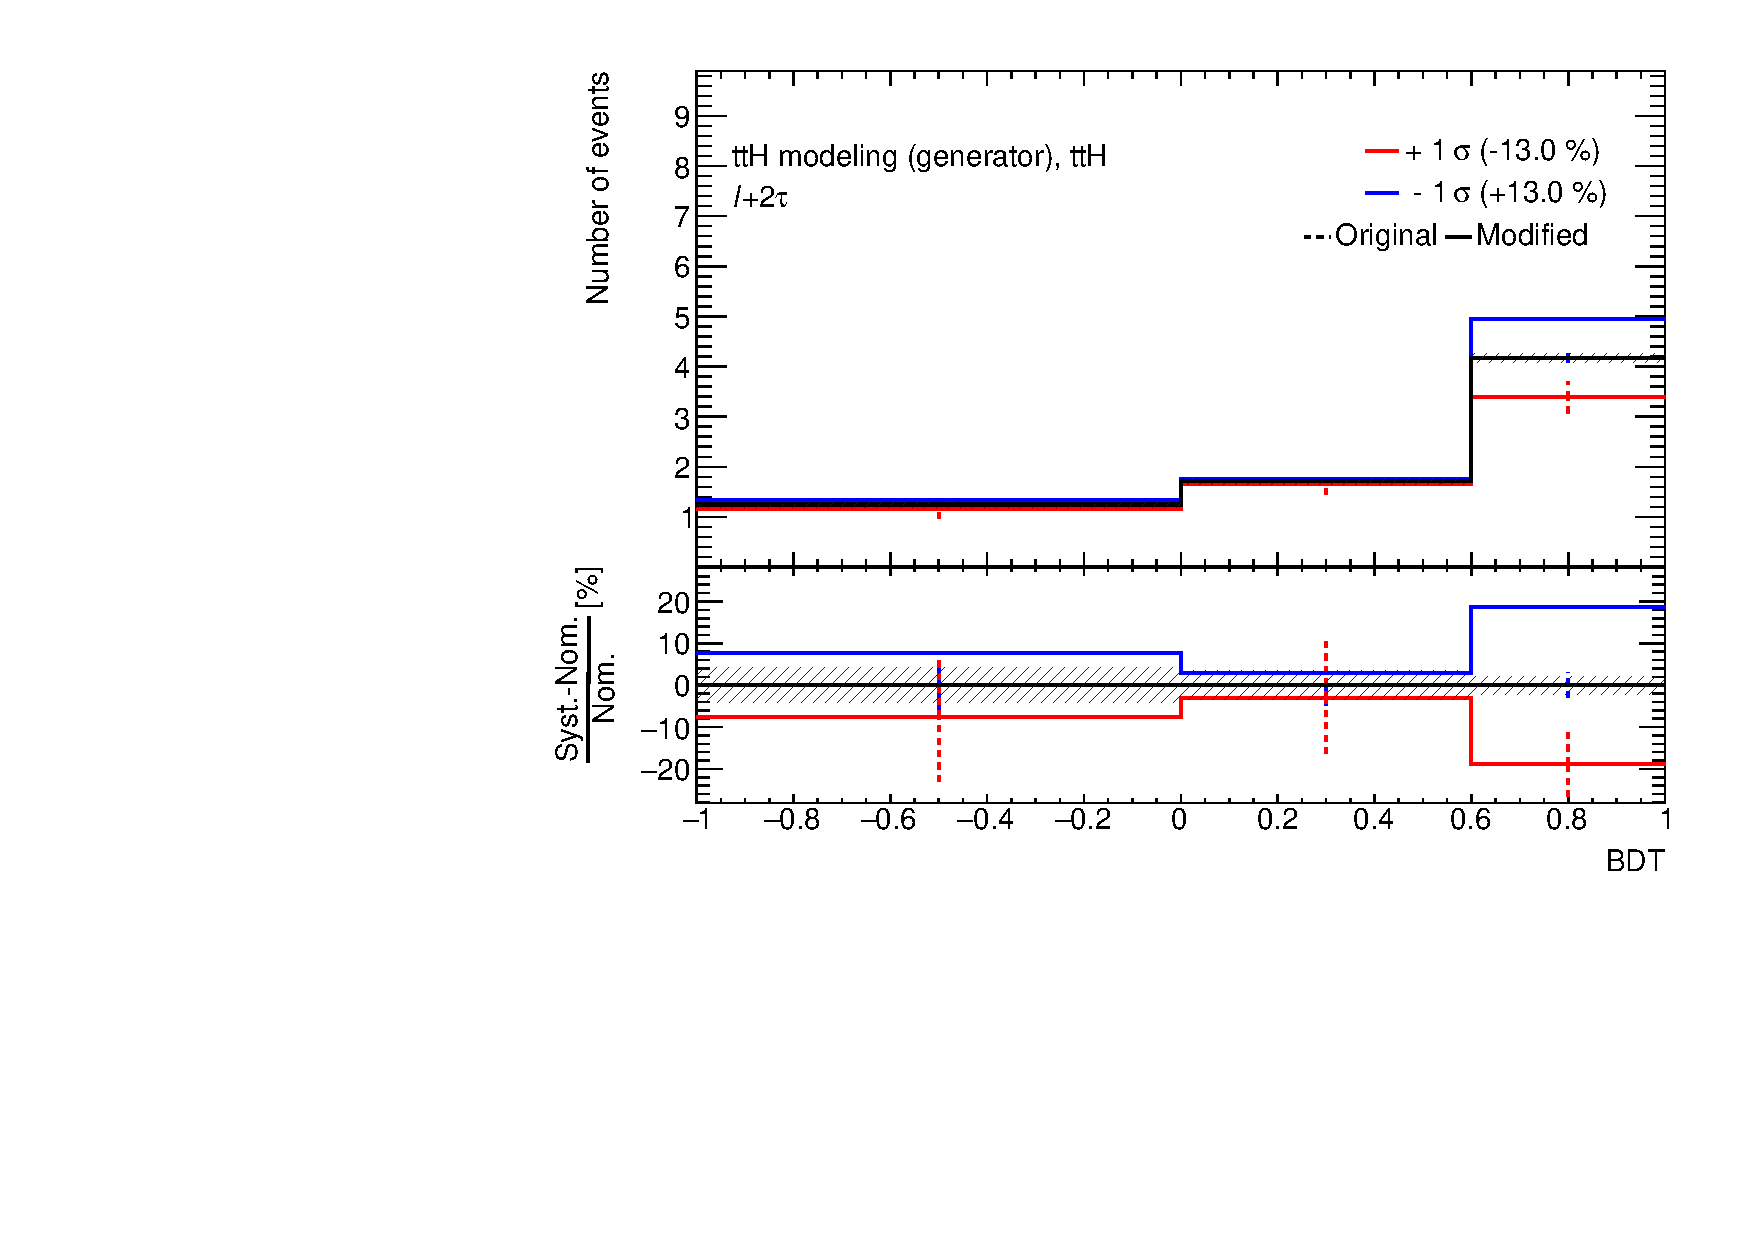
\includegraphics[width=0.32\textwidth, angle=-90, keepaspectratio]{fig/OneLepTwoTaus/Plots_tth-signal_MCsys.pdf}
  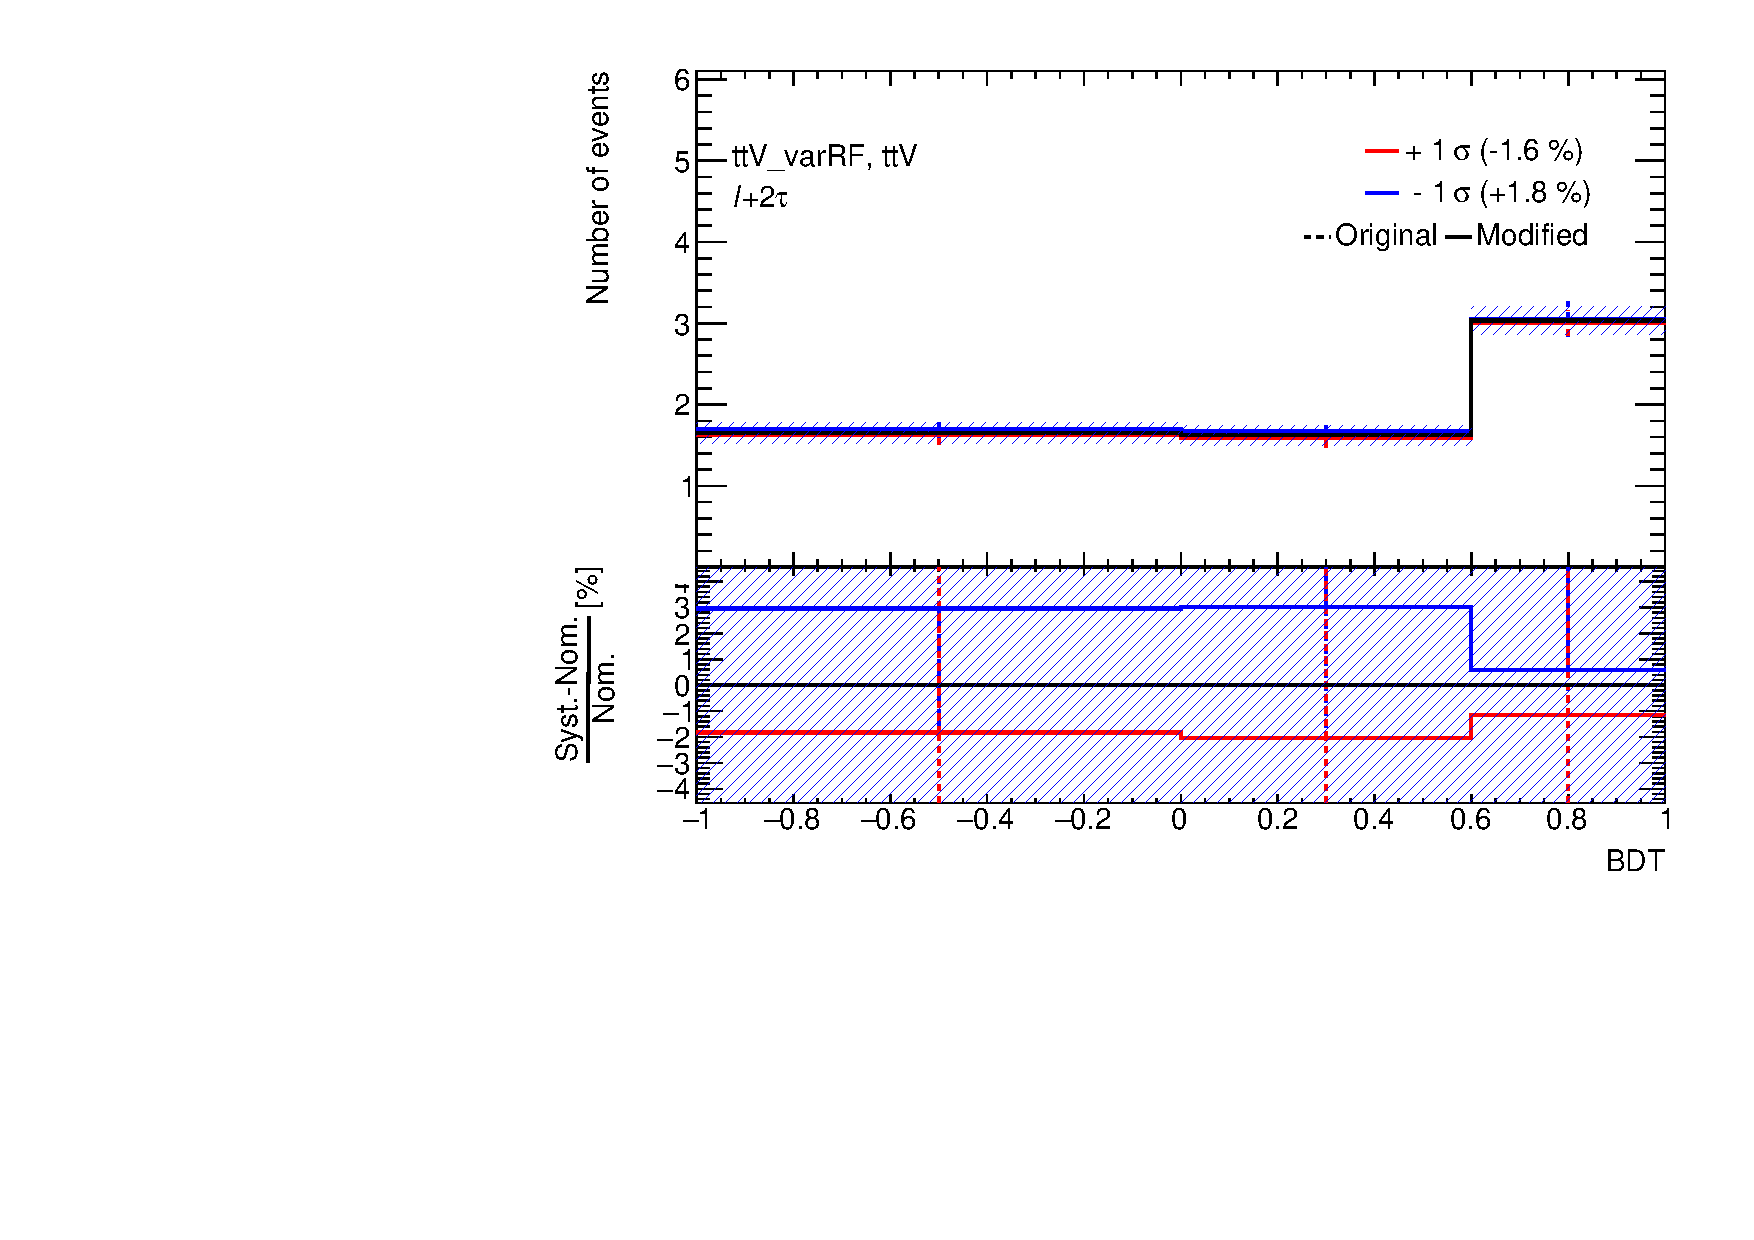
\includegraphics[width=0.32\textwidth, angle=-90, keepaspectratio]{fig/OneLepTwoTaus/Plots_ttV-signal_MCsys.pdf}
  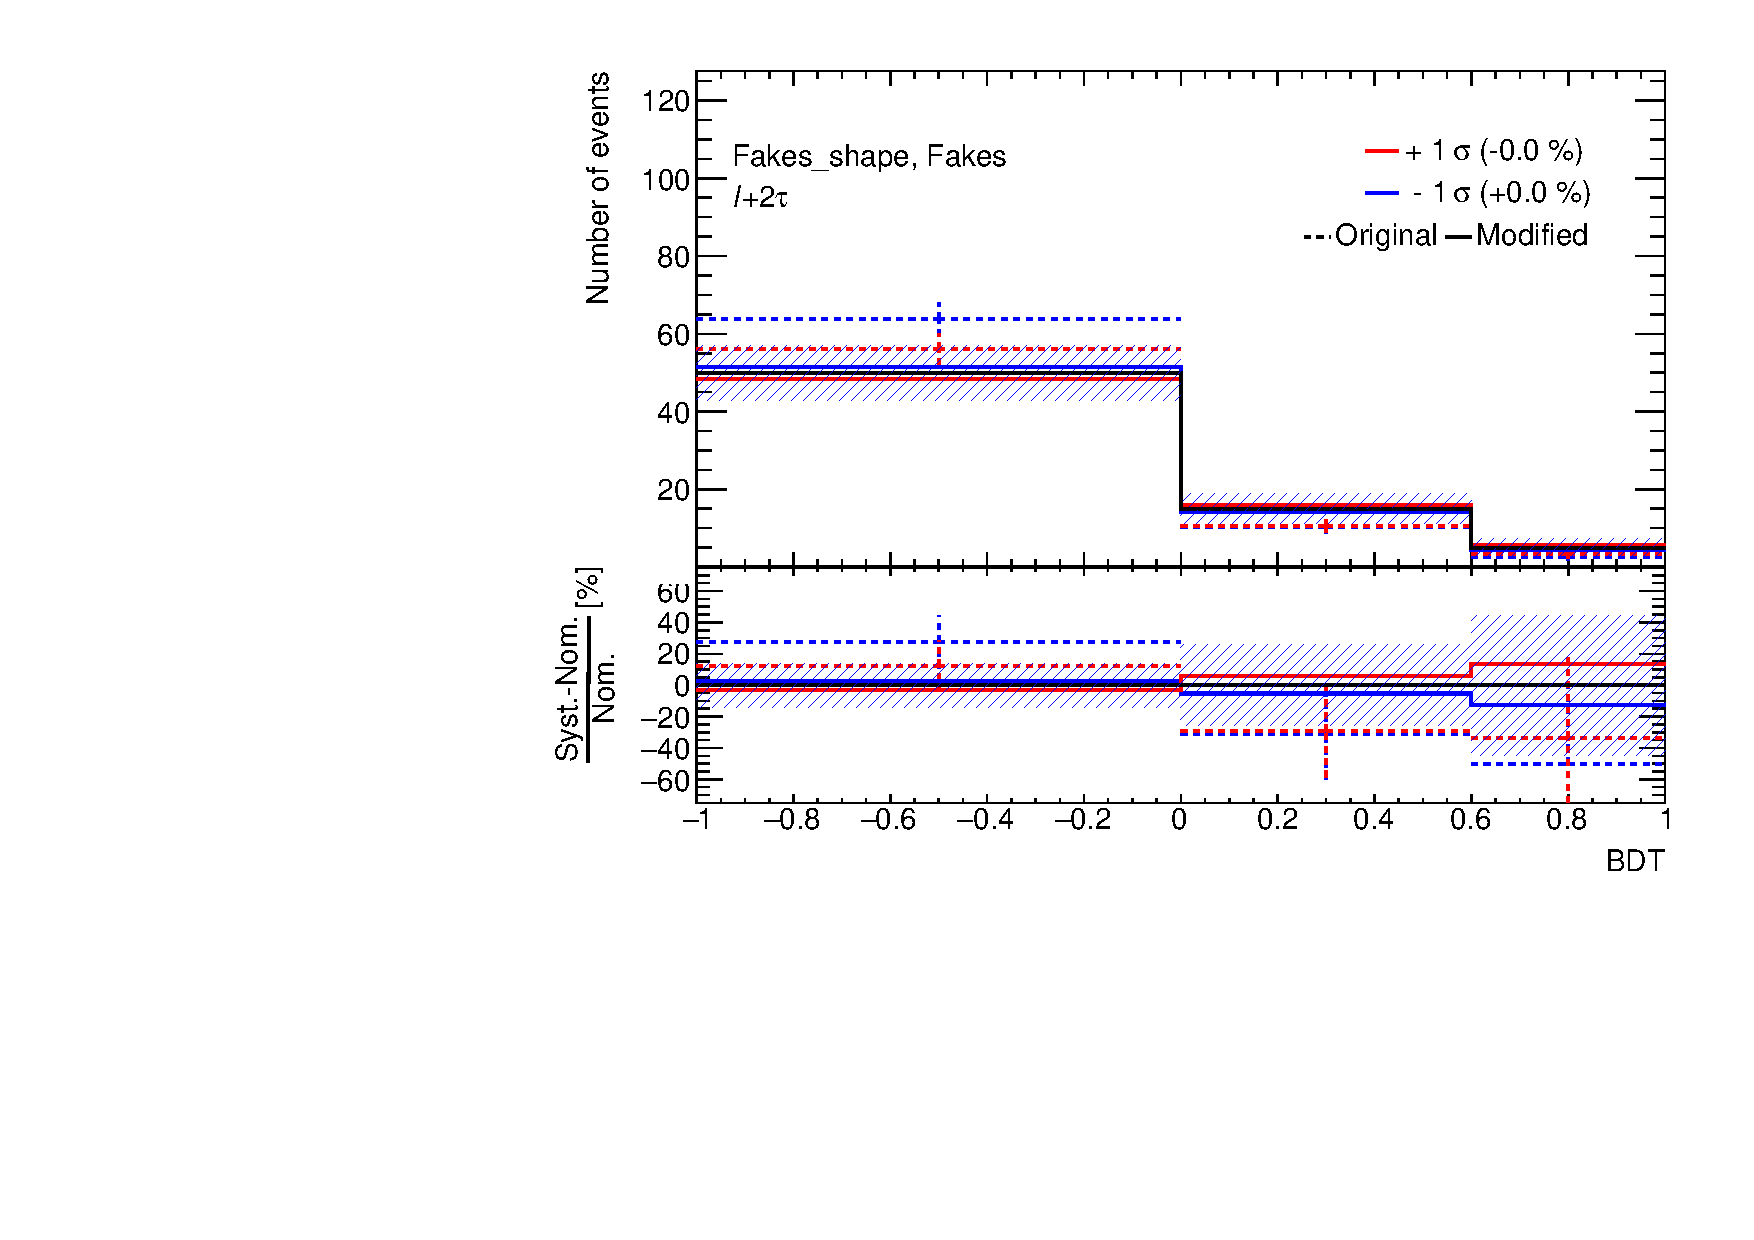
\includegraphics[width=0.32\textwidth, angle=-90, keepaspectratio]{fig/OneLepTwoTaus/h1l2tau_Fakes.pdf}
\end{center}
\caption{系统误差举例:$t\bar{t}h$产生子,部分子簇射参数和fakes形状误差。前两者同时影响接收度和形状,fakes形状误差利用$t\bar{t}$ MC估计。}
%\caption{The BDT shape systematic is estimated using different Monte Carlo generators including the SS/OS shape systematic from fakes. 
%which are compared for tth, ttV, and SS/OS with fakes from Monte Carlo events.
%({\bf update })
%}
\label{Fig:1l2tau.shapesys}
\end{figure}
